
\chapter{Vorgehensweise}

\section{Datengewinnung - Inferenz der Pose des Agenten}
\label{collect-data}

Zur Erzeugung der Trainingsdaten wird in jedem \texttt{step}-Aufruf des Simulators das dazugehörige Kamerabild der DuckieBots abgegriffen, mit dem korrespondierenden Label versehen und anschließend abgespeichert. Das Label beinhaltet hierbei folgende Informationen:

\begin{enumerate}
	\item Kürzester Abstand $d$ zur rechten Fahrbahnmarkierung
	\item Winkeldifferenz $\Theta$ zwischen Orientierung des DuckieBots und der Fahrbahn
	\item Name der Kachelart, auf der sich der DuckieBot zur Zeit der Aufnahme des Kamerabildes befindet
\end{enumerate}

Die Labelinformationen können dabei direkt aus dem DuckieTown-Simulator entnommen bzw. berechnet werden. Des Weiteren kann gesteuert werden, wie viele Kamerabilder aufgenommen werden sollen. \\

Im folgenden werden wir auf zwei verschiedene Ansätze eingehen, die wir zur Gewinnung der Daten verfolgt haben:

\subsection{Ansatz 1 - PID-Fahrt ohne Neuplatzierung des Agenten:}

Der DuckieBot wird mittels eines PID-Reglers gesteuert, so dass er die Mitte der rechten Fahrspur hält und den Streckenverlauf der Fahrbahn verfolgt. Dabei wird der DuckieBot auf einer zufälligen befahrbaren Kachel der Umgebung platziert. Die Orientierung des DuckieBots  wird hierbei ebenfalls zufällig ausgewählt.

\subsection{Ansatz 2 - PID-Fahrt mit Neuplatzierungen des Agenten:}

Bei diesem Ansatz wird der DuckieBot ebenfalls mit Hilfe eines PID-Reglers (wie in Ansatz 1 beschrieben) gesteuert. Der Unterschied hierbei ist, dass der DuckieBot nach einer gewissen Anzahl von \texttt{step}-Aufrufen des Simulators neu platziert wird. Die Platzierung des DuckieBots erfolgt hierbei ebenfalls zufällig, nach dem im Ansatz 1 beschriebenen Verfahren.

\section{Datengewinnung - Direkte Inferenz des Steuerbefehls}

Die Gewinnung der Kamerabilder des DuckieBots läuft hierbei analog, wie im Abschnitt \ref{collect-data} beschrieben ab. Die abgegriffenen Kamerabilder werden anschließend mit folgenden Informationen gelabelt:

\begin{enumerate}
	\item Geschwindigkeit $v$
	\item Winkelgeschwindigkeit $\omega$
	\item Name der Kachelart, auf der sich der DuckieBot zur Zeit der Aufnahme des Kamerabildes befindet
\end{enumerate}


Der optimale Steuerbefehl (bestehend aus $v$ und $\omega$) wird hierbei durch ein sogenanntes Expertensystem zu Verfügung gestellt. Der Name der Kachelart, auf der sich der DuckieBot zur Zeit der Aufnahme befindet, kann wieder direkt aus dem Simulator abgegriffen werden. \\

Hierbei haben wir ebenfalls zwei verschiedene Ansätze zur Gewinnung der Daten verfolgt, auf die wir im folgenden eingehen werden:

\subsection{Ansatz 1 - Expertenfahrt ohne Neuplatzierung des Agenten:}

Der DuckieBot wird mit Hilfe des vom Expertensystem vorhergesagten Steuerbefehls gesteuert. Er wird hierbei ebenfalls zu Beginn auf einer zufälligen Kachel platziert, mit einer ebenfalls zufällig ausgewählten Orientierung.

\subsection{Ansatz 2 - Expertenfahrt mit Neuplatzierung des Agenten:}

Bei diesem Ansatz wird der DuckieBot ebenfalls mit dem vom Expertensystem vorhergesagten Steuerbefehls navigiert. Jedoch wird nach einer gewissen Anzahl von \texttt{step}-Aufrufen des Simulators, eine zufällige Neuplatzierung des DuckieBots vorgenommen.


\section{Netzwerkarchitektur}

Die entworfene Netzwerkarchitektur ist sowohl für die Inferenz der Pose des Agenten als auch für die direkte Inferenz des Steuerbefehls identisch.
Für die Realisation des Netzwerkes haben wir \href{https://www.tensorflow.org/}{TensorFlow} verwendet. TensorFlow ist ein von Google entwickeltes Framework für maschinelles Lernen und Künstliche Intelligenz \cite{bigdata}. \\

Unsere Netzwerkarchitektur besteht aus 12 Schichten: einer Normalisierungsschicht, fünf Faltungsschichten, 2 Dropoutschichten, einer Flattenschicht und drei Fully-Connected-Schichten.
Dabei haben wir uns an einer bereits vorhanden Netzwerkarchitektur eines NVIDIA-Papers orientiert. Der Titel des Paper lautet: \glqq End to End Learning for Self-Driving Cars\grqq{} und kann unter \href{https://arxiv.org/pdf/1604.07316.pdf}{https://arxiv.org/pdf/1604.07316.pdf} gefunden werden.
Eine schematische Darstellung der Netzarchitektur ist in Abbildung \ref{network-architecture} dargestellt. \\

Im folgenden werden wir den Aufbau der Netzarchitektur näher erläutern:

\subsection{Normalisierungsschicht}
Die Grundidee der Normalisierungsschicht besteht darin, die Ausgabe einer Aktivierungsschicht zu normalisieren, wodurch die Konvergenz während des Trainingsprozesses verbessert wird. \cite{tensorflow}

\subsection{Faltungsschichten}
Nach der Normalisierungsschicht folgen die einzelnen Faltungsschichten. Diese sind für die Extraktion von Bildmerkmalen zuständig. \\

Die erste Faltungsschicht nutzt hierbei 24 verschiedene Filter (Kernel) der Größe 5x5 mit einer 2x2 Schrittbreite (stride) unter der Berücksichtigung der Bildränder (padding). Als Aktivierungsfunktion wird die ELu verwendet. Des Weiteren wird ein L2-Kernel-Regularizer eingesetzt, damit das Overfitting des Modells minimiert wird \cite{tensorflow2}.  \\ 
Das 5x5 große Fenster fährt dann über das Eingabebild und wendet alle 24 Filter auf den momentanen Bildausschnitt an. Jeder dieser Filter konzentriert sich dabei auf ein bestimmtes Bildmerkmal. \\

Die zweite Faltungsschicht nutzt 36 verschiedene Kernel. Die restlichen Parameter sind identisch zur ersten Faltungsschicht. \\

Die dritte Faltungsschicht nutzt 48 verschiedene Filter. Auch hier sind die restlichen Parameter identisch zur ersten Faltungsschicht. \\

Die vierte Faltungsschicht nutzt 64 verschiedene Kernel der Größe 3x3 mit einer 1x1 Schrittbreite, jedoch werden hier die Bildränder nicht berücksichtigt. Die restlichen Parameter sind wieder identisch zur ersten Faltungsschicht. \\

Die fünfte und letzte Faltungsschicht ist identisch zur vierten Faltungsschicht.

\subsection{Flattenschicht}

Nach den Faltungsschichten folgt eine sogenannte Flattenschicht, die dafür zuständig ist, die mehrdimensionale Ausgabe der Faltungsschichten  in eine eindimensionale Repräsentation zu überführen. \cite{hhu}

\subsection{Dropoutschichten}

Zwischen der vierten und der fünften Faltungsschicht befindet sich eine Dropoutschicht, sowie nach der Flattenschicht. \\ Die Dropoutschichten dienen zur Minimierung der Gefahr einer Überanpassung des Modells an die Trainingsdaten. Dabei wird beim Training des Modells eine vorher spezifizierte Anzahl von Neuronen ausgeschaltet, die dann im kommenden Berechnungsschritt nicht berücksichtigt werden. \cite{wiki2}

\subsection{Fully-Connected-Schichten}

Nach den Faltungsschichten folgen anschließend drei Fully-Connected-Schichten die uns schlussendlich die geschätzte Distanz $d$ und geschätzte Winkeldifferenz $\Theta$ liefern.
\vspace{0.6cm}
\begin{figure}[H]
	\centering
	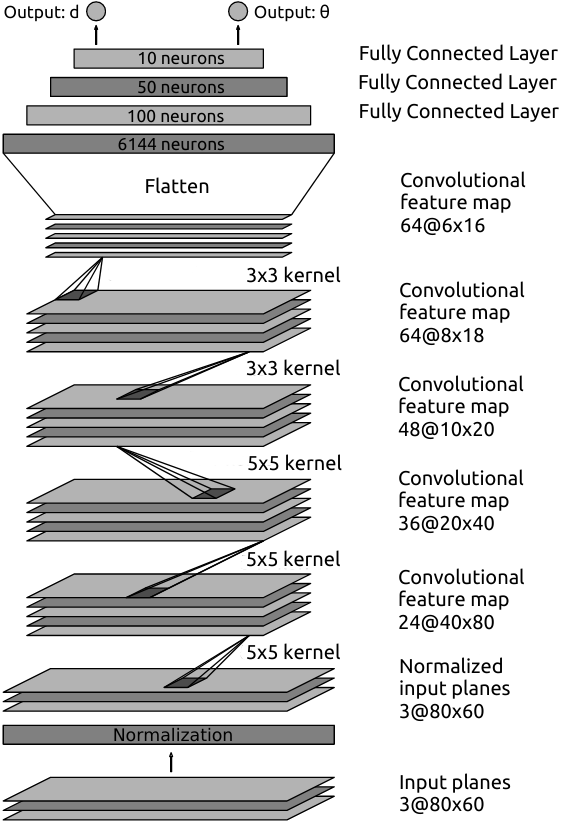
\includegraphics[width=0.75\textwidth]{kapitel4/images/network_architecture.png}
	\caption{Schematische Darstellung der Netzwerkarchitektur}
	\label{network-architecture}
	\vspace{0.2cm}
	\quelle\url{https://d3i71xaburhd42.cloudfront.net/0e3cc46583217ec81e87045a4f9ae3478a008227/5-Figure4-1.png}
\end{figure}

Das Netzwerk nimmt das Kamerabild des DuckieBots als Eingabe entgegen, wobei das obere drittel des Kamerabildes entfernt wurde. Dies hat den Vorteil, dass somit nur die relevanten Informationen für das Netzwerk im Kamerabild enthalten sind, wodurch sich das Training des Netzwerks verbessert. Das Netzwerk verarbeitet dann das eingehende Kamerabild und liefert anschließend die geschätzte Pose, bestehend aus dem kürzestem Abstand $d$ zur rechten Fahrbahnmarkierung sowie der Winkeldifferenz $\Theta$ zwischen Orientierung des DuckieBots und der Fahrbahn.


\section{Lernprozess}

Für den Lernprozess wird das überwachte Lernen als Lernverfahren eingesetzt. Zu Beginn des Lernprozesses werden zunächst die Hyperparameter des Modells festgelegt:
\vspace{-0.4cm}
\begin{center}
	\begin{tabular}[t]{|l|l|}
		\hline
		\textbf{Lerngeschwindigkeit} & 0.0002 \\
		\hline
		\textbf{Batch Größe} & 32 \\
		\hline
		\textbf{Optimizer} & Adam \\
		\hline
		\textbf{Anzahl Epochen} & 50 \\
		\hline
		\textbf{Verlustfunktion} & MSE \\
		\hline
	\end{tabular}
\end{center}

Anschließend wird einer der zuvor vorbereiteten Datensätze geladen, womit dann das Training des Modells erfolgt. \\

Der Hauptmechanismus des Trainings stellt eine Feedback-Schleife dar. Die grundlegende Idee dabei ist, dass wir dem Modell die aufgenommenen Kamerabilder zeigen und uns die Vorhersagen des Modells merken. Anschließend können wir die Korrektheit der erhalten Vorhersagen prüfen und den Fehler im Bezug zum tatsächlichen Wert ermitteln. Daraufhin erfolgt im Modell eine Anpassung der einzelnen Gewichte der Neuronen (durch den Backpropagation-Mechanismus), mit dem Ziel bessere Vorhersagen treffen zu können. Anschließend wird der Vorgang wiederholt. Ein einzelner Durchlauf der  Feedback-Schleife wird dabei als eine Epoche bezeichnet. Je größer die Anzahl der Epochen eines künstlichen neuronalen Netzes ist, desto länger wurde es trainiert. Zum Schluss wird das trainierte Modell abgespeichert, damit es in den Simulator integriert werden kann.

